\chapter{Binned \KlPiPi vs \4Pi yields }

\section{Overview}
The values for $MM_i$ are obtained using:
\begin{equation}
MM_i = (N_i^{meas} - B_i^{peak} - B_i^{flat} - B_i^{cont})/ \epsilon_i
\end{equation}
$MM_i$ : absolute number of \4Pi vs \KlPiPi events in bin i. This is the quantity that enters the fit for $F_+$.\\
$N_i^{meas}$ : total number of reconstructed and selected events in bin i. \\
$B_i^{peak}$ : number of reconstructed and selected peaking bkg. events in bin i.\\
$B_i^{flat}$ : number of reconstructed and selected flat bkg. events in bin i.\\
$B_i^{cont}$ : number of reconstructed and selected continuum bkg. events in bin i.\\
$\epsilon_i$ : reconstruction and selection efficiency for \4Pi vs \KlPiPi events in bin i. \\



\section{Raw number of selected \4Pi vs \KlPiPi events }
The selection of \4Pi vs \KlPiPi was done as outlined in Chris' report. The resulting numbers are listed below.\\
\begin{table}[!h]
	\begin{center}
	\begin{tabular}{c| l}
		bin i & $N^{meas}_i\ \pm \sqrt{N^{meas}_i}$  \\
		\hline 
		\hline
1 & 172 $\pm$ 13.11 \\ 
2 & 71 $\pm$ 8.43 \\ 
3 & 60 $\pm$ 7.75 \\ 
4 & 25 $\pm$ 5 \\ 
5 & 59 $\pm$ 7.68 \\ 
6 & 32 $\pm$ 5.66 \\ 
7 & 71 $\pm$ 8.43 \\ 
8 & 99 $\pm$ 9.95 \\ 
\end{tabular}
\end{center}
\caption{\textit{Number $N^{meas}_i$ of reconstructed \4Pi vs \KlPiPi events summed over bin i and -i. The errors are taken as $\sqrt{N^{meas}_i}$.}}
\end{table}


\section{Determination of number of peaking background events}
\label{sec:klpeak}
Three decays are identified as peaking bkg (peaking in missing mass squared) for \KlPiPi vs \4Pi using the gen MC (see Figure \ref{fig:missmasssq}):
\begin{itemize}
\item \KlPiPi vs \KsPiPi : 8\% of the events in the signal window
\item \KsPiPi vs \4Pi : 1.9\% of the events in the signal window
\item \KsPiPi vs \KsPiPi : 0.3\% of the events in the signal window
\end{itemize}
(signal window: $0.2\, GeV^2$ < miss. mass sq < $0.3\, GeV^2$). Due to the very low contribution the \KsPiPi vs \KsPiPi bkg is being neglected.\\
\begin{figure}[!h]
	\vspace*{-0.cm}
	\begin{center}
		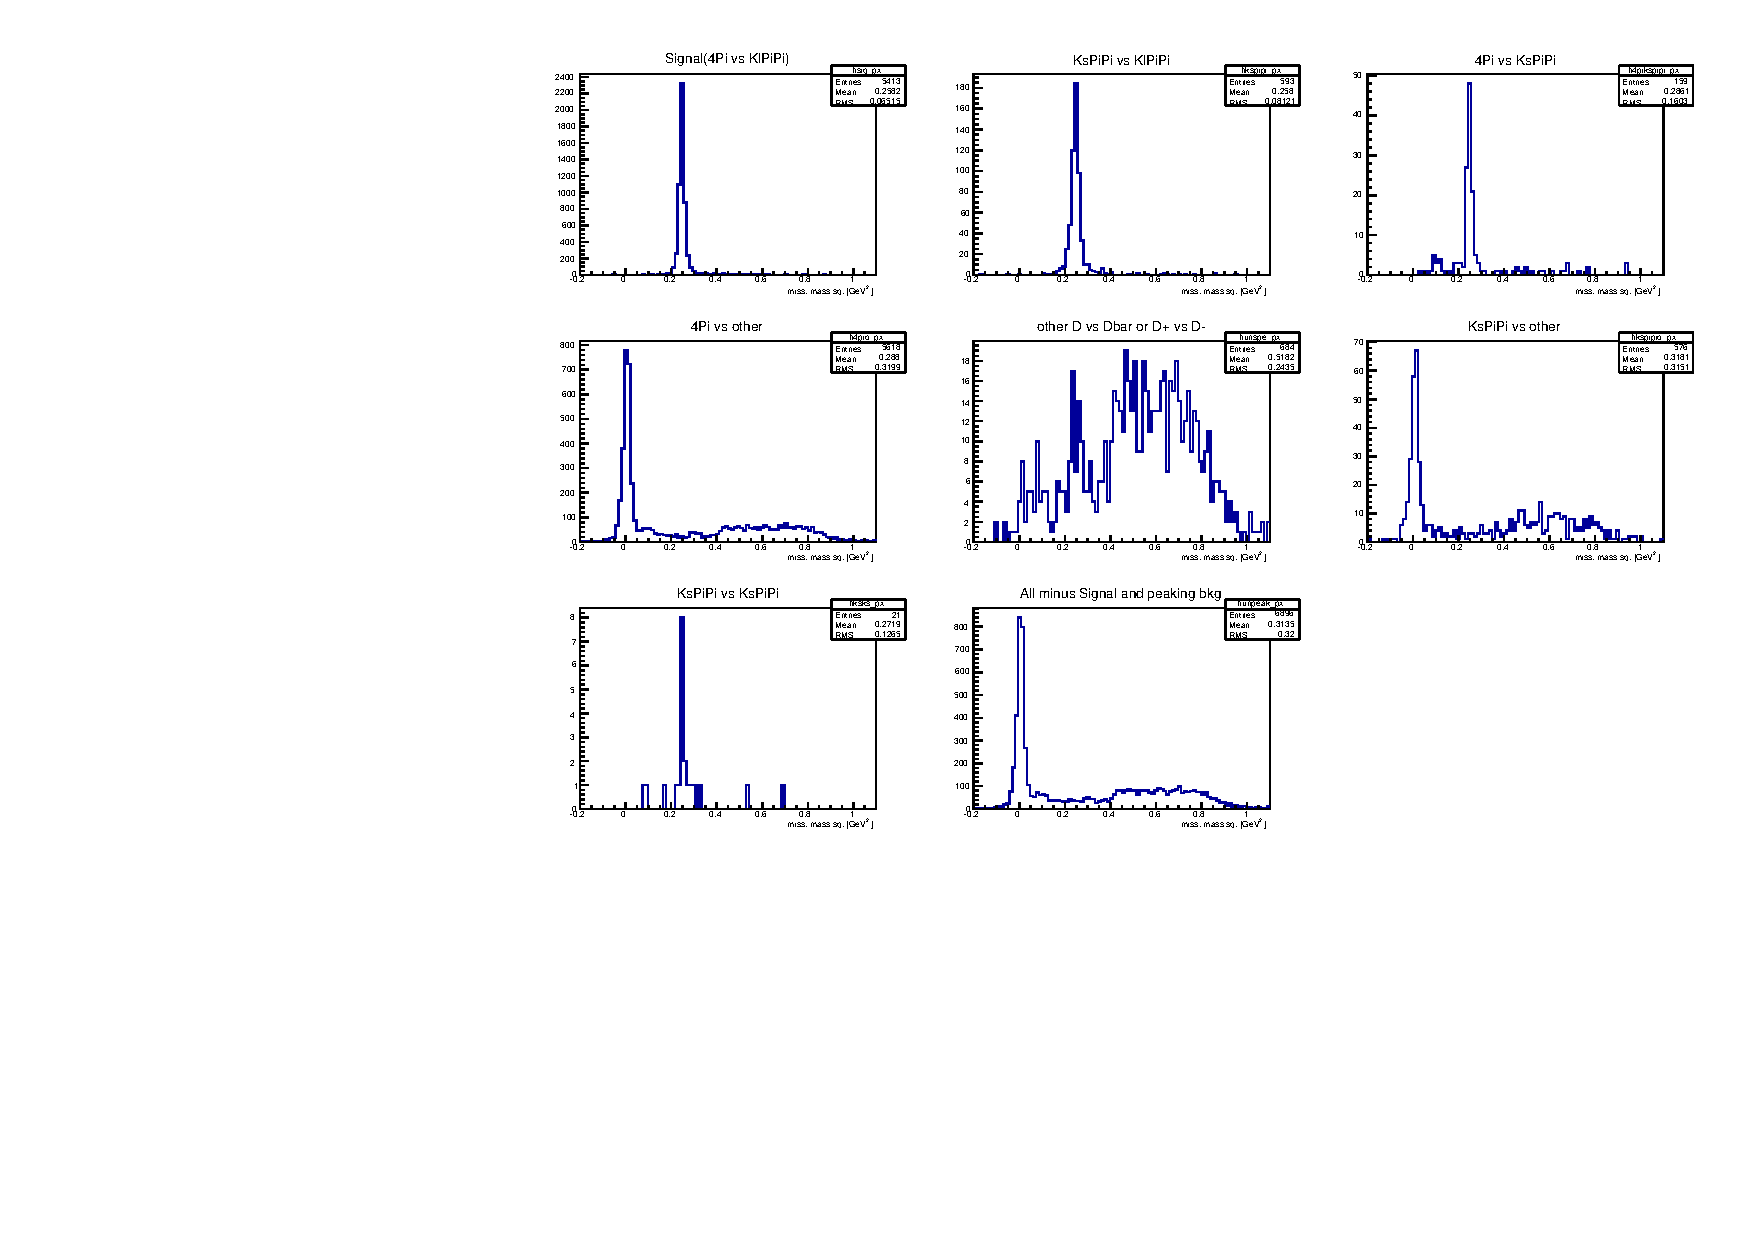
\includegraphics[width=1.\textwidth]{missmasssq.pdf}
		\vspace*{-1.5cm}
	\end{center}
	\caption{\textit{Missing mass squared distribution of different types of events reconstructed as  \KlPiPi vs \4Pi according to the gen MC.}}
	\label{fig:missmasssq}
\end{figure}\\
As for the \KsPiPi vs \4Pi the number of peaking bkg events per bin is determined from
\begin{equation}
B_i^{peak} = B_{tot}^{peak} \cdot a_i^{peak}
\end{equation}
for both bkgs separately, where $B_{tot}^{peak}$ denotes the total number of peaking bkg events in the selected data sample and $a_i^{peak}$ the percentage of peaking bkg  events in bin i.\\

\subsection{Total number of peaking background events in selected data sample}
The total number of peaking bkg events in the selected sample is determined using the generic MC. The same reconstruction and selection as to the data is applied to the generic MC. This results in $98 \pm 9.90$ and $419 \pm 20.47$ selected \KlPiPi vs \KsPiPi events in the lumix10 and lumix20 sample respectively and $15 \pm 3.87$ and $90 \pm 9.49$ \KsPiPi vs \4Pi events (the errors are taken to be the sqrt of the yields).
These numbers are then scaled appropriately to give the expected number of total bkg events in the reconstructed data sample and no error on the scaling factors is assumed.
\begin{equation}
B_{tot}^{peak}(\KlPiPi\, vs\, \KsPiPi) = 35.51 
\end{equation}
and 
\begin{equation}
B_{tot}^{peak}(\KsPiPi\, vs\, 4\pion) = 9.42
\end{equation}
Since the branching fraction of $\D \rightarrow \KlPiPi$ is unknown, the fraction of \KlPiPi events in the gen MC sample can't be completely accurate. This will be accounted for by applying a systematic to the number of events obtained from the gen MC (by assuming that the branching fraction used by CLEO is 20\% too small/big).\\

\subsection{Distribution of \KlPiPi vs \KsPiPi background events over bins}
\label{sec:klclean}
As for the \KsPiPi vs \KsPiPi bkg in \KsPiPi vs \4Pi the distribution of \KlPiPi vs \KsPiPi events per bin is determined by applying a 'reversed \KS veto' on the data. The gen MC sample suggests that after the reversed \KS veto sample contains:
\begin{itemize}
\item \KlPiPi vs \KsPiPi : 92\%
\item flat events: 5\% 
\item \KlPiPi vs \4Pi : 1.5\%
\item \KsPiPi vs \KsPiPi : 1.5\%
\end{itemize} 
The last two are neglected for now (a systematic will be appointed later).\\
\\
In order to obtain the distribution of \KlPiPi vs \KsPiPi events over the bins, the contribution of flat bkg events is estimated as in Section \ref{sec:flat} and removed from the data.\\ 

\subsubsection{Selection-bias}	
Unfortunately 'reversed \KS veto' introduced a bias in the distribution of expected \KlPiPi vs \KsPiPi events over the bins. \\
To compensate for this bias the values for $a_i^{peak}$ are being weighted with the ratio of reversed \KS veto over the \KS veto efficiencies determined from the \KlPiPi vs \KsPiPi signal MC sample.\\

\subsection{Distribution of \KsPiPi vs \4Pi background events over bins}
The 'true' distribution of \KsPiPi vs \4Pi events in phasespace is taken from the results of the \KsPiPi vs \4Pi analysis, namely the values of Table \ref{tab:MMKs}.\\


\subsection{Resulting number of peaking background events in selected data sample}
Applying these scaling values to the factors $a_i$ yields the total amount of peaking bkg contamination in the data sample listed below.

\begin{table}[!h]
	\begin{center}
		\begin{tabular}{c| c}
			bin i & $B^{peak}_i(\KlPiPi\, vs\, \KsPiPi)$    \\
			\hline 
			\hline
1 & 12.267 $\pm$ 3.5 $\oplus$ 1.06294 \\ 
2 & 3.81339 $\pm$ 2 $\oplus$ 0.666631 \\ 
3 & 2.85437 $\pm$ 2 $\oplus$ 0.608983 \\ 
4 & 1.48931 $\pm$ 1.5 $\oplus$ 0.442086 \\ 
5 & 3.68781 $\pm$ 2 $\oplus$ 0.63337 \\ 
6 & 1.72474 $\pm$ 1.5 $\oplus$ 0.415589 \\ 
7 & 4.03395 $\pm$ 2 $\oplus$ 0.709566 \\ 
8 & 5.63443 $\pm$ 2.5 $\oplus$ 0.804392 \\ 
	\end{tabular}
	\end{center}
	\caption{\textit{Number of \KsPiPi vs \KlPiPi background events per bin in the data sample.The first error is the Poisson error on the yields, the second error comes from the sys- tematic uncertainty on the distribution over the bins. }}
	\vspace*{1cm}
\end{table}

\begin{table}[!h]
	\begin{center}
		\begin{tabular}{c| c}
			bin i & $B^{peak}_i(\KsPiPi\, vs\, 4\pion)$    \\
			\hline 
			\hline
1 & 1.32987 $\pm$ 1 $\oplus$ 0.302816 \\ 
2 & 0.856693 $\pm$ 1 $\oplus$ 0.227813 \\ 
3 & 0.707903 $\pm$ 0.5 $\oplus$ 0.194539 \\ 
4 & 0.438423 $\pm$ 0.5 $\oplus$ 0.146814 \\ 
5 & 2.38231 $\pm$ 1.5 $\oplus$ 0.349486 \\ 
6 & 0.910659 $\pm$ 1 $\oplus$ 0.220425 \\ 
7 & 1.19564 $\pm$ 1 $\oplus$ 0.258476 \\ 
8 & 1.59349 $\pm$ 1.5 $\oplus$ 0.294614 \\ 

	\end{tabular}
	\end{center}
	\caption{\textit{Number of \4Pi vs \KsPiPi background events per bin in the data sample. The first error is the Poisson error on the yields, the second error comes from the sys- tematic uncertainty on the distribution over the bins. }}
	\vspace*{1cm}
\end{table}

\section{Determination of number of flat and continuum background events}
The total number of flat bkg events and continuum bkg events is determined using a form of the 'Powell method'.\\
In this method the missing mass squared region is divided into three regions: the lower region ($0.05\,GeV^2$ - $0.2\,GeV^2$), the signal region ($0.2\,GeV^2$ - $0.3\,GeV^2$) and the higher region ($0.45\,GeV^2$ - $0.8\,GeV^2$).
 The raw event yield $D_i$ in rach sideband i is expressed as:
\begin{equation}
D_i = T_{Si} + T_{Pi} + T_{Ci} + T_{Fi}
\end{equation}
where $T_{Si}$ denotes the raw signal yield in sideband i, $T_Pi$ the raw yields of peaking bkg events, $T_Fi$ the raw yields of flat bkg events and $T_{Ci}$ the raw yields of continuum events.\\
Since the raw peaking bkg yield has been calculated earlier, we get a system of three equations, one for each region of missing mass squared:
\begin{equation}
D_i -T_{Pi} = T_{Si} + T_{Ci} + T_{Si}
\end{equation}
By assuming that the ratio of numbers of events in each sideband is modulated correctly by the MC samples - e.g. $T_{S1} = \frac{m_{S1}}{m_{S2}} T_{S2}$, where $m_{Si}$ is the number of signal events in the MC sample - these three equations can be expressed in terms of three unknowns:
\begin{equation}
D_1 -T_{P1} =  \frac{m_{S1}}{m_{S2}} T_{S2}  + T_{C1} + \frac{m_{F1}}{m_{F3}} T_{F3}  \\
\end{equation}
\begin{equation}
D_2 -T_{P2} =   T_{S2}  + \frac{m_{C2}}{m_{C1}} T_{C1} + \frac{m_{F2}}{m_{F3}} T_{F3} \\
\end{equation}
\begin{equation}
D_3 -T_{P3} =  \frac{m_{S1}}{m_{S3}} T_{S2}  + \frac{m_{C3}}{m_{C1}} T_{C1} +  T_{F3} \\
\end{equation}
This system can be solved by a simple matrix inversion and thus the number of continuum and flat bkg events in the signal window found (Chris thesis Section 3.6.3). \\
The difference to method described in Chris thesis is that instead of dividing the flat bkg into 'peaking in low sideband' and 'peaking in high sideband' the bkg is divided into continuum and flat bkg.

%The total number of continuum events is extrapolated from the CLEO continuum MC sample. This results in 38.93 $\pm$ 7.70 continuum events in the signal window of our data sample.\\
%Furthermore the continuum bkg is assumed to be flat in phasespace, so the 38 events are distributed across the bins according to Table \ref{tab:a_i}. This results in the following number of continuum events per bin:
%
%\begin{table}[!h]
%	\begin{center}
%		\begin{tabular}{c| l}
%			bin i & $B^{cont}_i$   \\
%			\hline 
%			\hline
%1 & 12.87 $ \pm$ 2.55 \\ 
%2 & 4.44 $ \pm$ 0.88 \\ 
%3 & 2.49 $ \pm$ 0.49 \\ 
%4 & 2.30 $ \pm$ 0.45 \\ 
%5 & 5.19 $ \pm$ 1.03 \\ 
%6 & 3.15 $ \pm$ 0.62 \\ 
%7 & 3.28 $ \pm$ 0.65 \\ 
%8 & 5.22 $ \pm$ 1.03 \\ 
%	\end{tabular}
%	\end{center}
%	\caption{\textit{Number of continuum background events per bin in the data sample. }}
%\end{table}
%
%
%\section{Determination of number of flat background events}

This results in 42.07 flat bkg events in the data sample and 17.06 continuum events.\\
The continuum bkg is also assumed to be flat in phasespace, so the 17 events are distributed according to the area of the bins. This results in the following number of continuum events per bin:
\clearpage
\begin{table}[!h]
	\begin{center}
		\begin{tabular}{c| c}
			bin i & $B^{cont}_i$   \\
			\hline 
			\hline
1 & 5.63723 $\pm$ 2.5 \\ 
2 & 1.94538 $\pm$ 1 \\ 
3 & 1.08944 $\pm$ 1 \\ 
4 & 1.00759 $\pm$ 1 \\ 
5 & 2.27215 $\pm$ 1.5 \\ 
6 & 1.37909 $\pm$ 1.5 \\ 
7 & 1.43683 $\pm$ 1.5 \\ 
8 & 2.28738 $\pm$ 1.5 \
	\end{tabular}
	\end{center}
	\vspace*{-0.5cm}
	\caption{\textit{Number of continuum bkg events per bin in the data sample. The error is the Poisson error on the bin-yields.}}
\end{table}

The number of flat bkg events in bin i are then:
\begin{table}[!h]
	\begin{center}
		\begin{tabular}{c| c}
			bins & $B_i^{flat}$  \\
			\hline
1 & 13.9052 $\pm$ 4 \\ 
2 & 4.79864 $\pm$ 2 \\ 
3 & 2.6873 $\pm$ 1.5 \\ 
4 & 2.4854 $\pm$ 1.5 \\ 
5 & 5.60467 $\pm$ 2.5 \\ 
6 & 3.40177 $\pm$ 1.5 \\ 
7 & 3.5442 $\pm$ 1.5 \\ 
8 & 5.64223 $\pm$ 2.5 \\ 
\end{tabular}
\end{center}
\vspace*{-0.5cm}
\caption{\textit{Number of flat bkg events per bin in the data sample. The error is the Poisson error on the bin-yields.}}
\end{table} 

\section{Determination of the signal selection-efficiency}
The signal selection efficiency in each bin is determined using a sample of 50\,000 \KlPiPi vs \4Pi signal MC events. The results are listed below.
\begin{table}[!h]
	\begin{center}
		\begin{tabular}{c| c }
			bin & $\epsilon$ [ \%] \\
			\hline
1 & 0.27805 $\pm$ 0.00155862 \\ 
2 & 0.270163 $\pm$ 0.00262954 \\ 
3 & 0.2553 $\pm$ 0.00345042 \\ 
4 & 0.258504 $\pm$ 0.00360249 \\ 
5 & 0.262955 $\pm$ 0.00241227 \\ 
6 & 0.26856 $\pm$ 0.00311724 \\ 
7 & 0.266931 $\pm$ 0.00304808 \\ 
8 & 0.267617 $\pm$ 0.00241776 \\
			\end{tabular}
	\end{center}
	\vspace*{-0.5cm}
	\caption{\textit{Signal efficiency per bin.}}
\end{table} 
\clearpage
\section{Resulting $MM_i$}
Since $M_i$	and $M_{-i}$ are the same, the numbers are directly evaluated for the sum of $M_i$ and $M_{-i}$ and listed on the table below.
\begin{table}[!h]
	\begin{center}
		\begin{tabular}{c| c }
			bin & $MM_i$  \\
			\hline
1 & 134.113 $\pm$ 13.8788 $\oplus$ 0.751773 $\oplus$ 1.02659 \\ 
2 & 59.2287 $\pm$ 8.89065 $\oplus$ 0.576484 $\oplus$ 0.662635 \\ 
3 & 55.3925 $\pm$ 8.62598 $\oplus$ 0.748637 $\oplus$ 0.640571 \\ 
4 & 20.3397 $\pm$ 5.73716 $\oplus$ 0.283453 $\oplus$ 0.459255 \\ 
5 & 46.0104 $\pm$ 8.63545 $\oplus$ 0.422086 $\oplus$ 0.646829 \\ 
6 & 24.5822 $\pm$ 6.22456 $\oplus$ 0.285332 $\oplus$ 0.415563 \\ 
7 & 61.1564 $\pm$ 8.97011 $\oplus$ 0.698343 $\oplus$ 0.71385 \\ 
8 & 84.1326 $\pm$ 10.7023 $\oplus$ 0.76009 $\oplus$ 0.807176 \\ 
	\end{tabular}
\end{center}
\caption{\textit{$M_i$ + $M_{-i}$ The first error comes from the Poisson error on the raw data yields and the bkg yields and the second error from the systematic uncertainty on the peaking bkg distribution and the third from the signal reconstruction and selection efficiency.}}
\label{tab:MMKl}
\end{table} 

\section{Summary}
\begin{table}[!h]
	\begin{center}
		\begin{tabular}{c| c | c | c| c|c|c }
		bin & raw yields & $B^{peak}_i(\KlPiPi\, vs\, \KsPiPi)$ & $B^{peak}_i(\KsPiPi\, vs\, 4\pion)$ & $B_i^{cont}$ & $B_i^{flat}$ & signal  \\
		\hline 
		\hline
1 & 172 & 12.26 & 1.32 & 13.90 & 5.63 & 134.11 \\ 
2 & 71 & 3.81 & 0.85 & 4.79 & 1.94 & 59.22 \\ 
3 & 60 & 2.85 & 0.70 & 2.68 & 1.08 & 55.39 \\ 
4 & 25 & 1.48 & 0.43 & 2.48 & 1.00 & 20.33 \\ 
5 & 59 & 3.68 & 2.38 & 5.60 & 2.27 & 46.01 \\ 
6 & 32 & 1.72 & 0.91 & 3.40 & 1.37 & 24.58 \\ 
7 & 71 & 4.03 & 1.19 & 3.54 & 1.43 & 61.15 \\ 
8 & 99 & 5.63 & 1.59 & 5.64 & 2.28 & 84.13 \\	
		\end{tabular}
	\end{center}
	\caption{\textit{Summary of contributions to the raw yields per bin.}}
\end{table}
